\section{Introducción}

La plataforma Gough-Cappel es un robot paralelo de seis grados de libertad.
Está compuesto por seis actuadores prismáticos que conectan una plataforma
móvil con una base mediante cardanes en un extremo de los actuadores y por
juntas esféricas o cardanes en el extremo contrario. 

% TODO image here

Conocido en la literatura como la 
plataforma Gough-Stewart, su origen se remonta a mediados del sigo XIX.
Su invención está documentada en 1954 por Eric Gough 
\cite{gough} en Inglaterra como una máquina para 
evaluar la respuesta de llantas de aviones a diferentes 
condiciones de aterrizaje (figura \ref{fig: gough robot}). 
De manera independiente, Klaus Cappel inventó un simulador de vuelo (figura \ref{fig: cappel robot})
con la misma arquitectura y una solicitud de patente 
fue sometida en 1964.
La popularización de este diseño de robot es debido a D. Stewart 
por su publicación en 1965, que sorprendentemente presenta el
diseño de un simulador de vuelo que no asemeja a la 
plataforma Gough Stewart (figura \ref{fig: stewart robot}).

% http://www.parallemic.org/Reviews/Review007.html

% TODO Insert 3 images for the designs by Gough, Cappel, and Stewart

\begin{figure}[hb!]
    \centering
    \begin{subfigure}[b]{0.3\textwidth}
        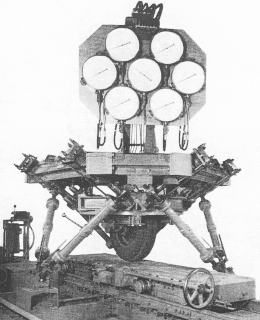
\includegraphics[width=\textwidth]{03_Reporte/img/GoughPlatform.png}
        \caption{Máquina universal diseñada por Gough. \cite{stewart}}
        \label{fig: gough robot}
    \end{subfigure}
    ~ %add desired spacing between images, e. g. ~, \quad, \qquad, \hfill etc. 
      %(or a blank line to force the subfigure onto a new line)
    \begin{subfigure}[b]{0.3\textwidth}
         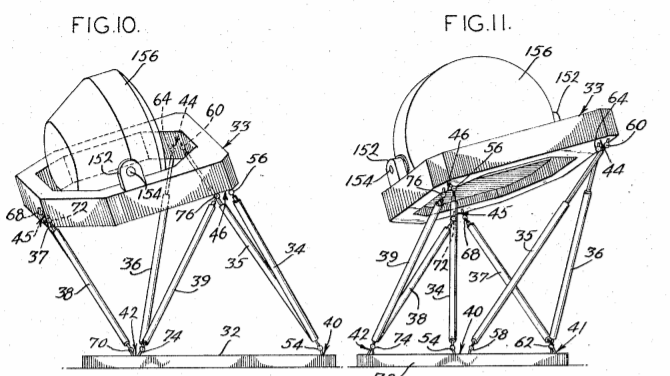
\includegraphics[width=\textwidth]{Cappel.png}
        \caption{Simulador de vuelo patentado por Cappel. \cite{cappel}}
        \label{fig: cappel robot}
    \end{subfigure}
    ~ %add desired spacing between images, e. g. ~, \quad, \qquad, \hfill etc. 
    %(or a blank line to force the subfigure onto a new line)
    \begin{subfigure}[b]{0.3\textwidth}
        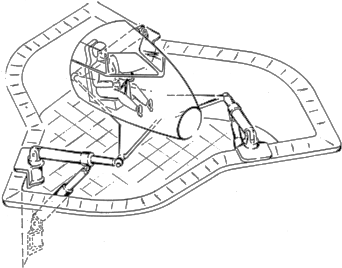
\includegraphics[width=\textwidth]{StewartPlatform.png}
        \caption{Simulador de vuelo propuesto por Stewart. \cite{stewart}}
        \label{fig: stewart robot}
    \end{subfigure}
    \caption{Iteraciones del robot paralelo.}\label{fig: parallel robots}
\end{figure}

